\section{Introduction}\label{sec:introduction}
\noindent\textbf{The problem in ordinary terms.}
Suppose that a continuous real function $f$ is available only through its
values at a prescribed collection of points in the square $Q=[-1,1]^2$.
We seek a polynomial that agrees with these values and can then be
evaluated elsewhere. Throughout this paper $\Pi_n$ denotes the vector
space of real polynomials in two variables whose total degree is at most
$n$. Here $n$ is a positive integer; the main theorems concern $n\geq2$.
Thus a monomial $x^py^q$ belongs to this space when $p,q$ are
nonnegative integers with $p+q\leq n$. For example,
\[
 \Pi_2=\operatorname{span}\{1,x,y,x^2,xy,y^2\}.
\]
The word ``total'' refers to the sum of the two exponents. Its triangular
index condition will also govern the frequency sums appearing later.
Counting the monomials by total degree gives
\[
 \dim\Pi_n=1+2+\cdots+(n+1)=\frac{(n+1)(n+2)}2.
\]
A choice of this many sample points gives a square system of linear
equations for the polynomial coefficients. The geometric placement of
the points determines whether that system has a unique solution.

For a function $g$ on $Q$, the notation $\|g\|_\infty$ means
$\max_{z\in Q}|g(z)|$ whenever $g$ is continuous. The space of all such
functions is written $C(Q)$. An interpolation operator $I_n$ maps $f$ to
the polynomial with the prescribed sampled values. Once uniqueness is
established, this operator is linear and reproduces every $p\in\Pi_n$:
$I_np=p$. Its norm is
\[
 \|I_n\|=\sup\{\|I_nf\|_\infty:f\in C(Q),\ \|f\|_\infty\leq1\}.
\]
This definition asks for the largest possible output size when the input
function has size at most one. Since interpolation uses only sampled
values, it also measures how those values can combine between nodes.

Polynomial interpolation replaces data at finitely many points by a polynomial.
Its usefulness depends on two questions: how well can polynomials approximate
the function, and how much can interpolation magnify errors in the data?
The Lebesgue constant measures the second effect. If $I_n$ denotes an
interpolation operator and $\Lambda_n=\|I_n\|$, then
\begin{equation}\label{eq:lebesgue-inequality}
 \|f-I_nf\|_\infty\leq (1+\Lambda_n)
       \inf_{p\in\Pi_n}\|f-p\|_\infty.
\end{equation}
\noindent\textbf{Why this estimate links approximation and stability.}
Fix any $p\in\Pi_n$. Reproduction and linearity give
\[
 f-I_nf=(f-p)-I_n(f-p),
 \qquad
 \|f-I_nf\|_\infty\leq(1+\|I_n\|)\|f-p\|_\infty.
\]
Taking the infimum over $p$ proves
\eqref{eq:lebesgue-inequality}. The infimum is the best error that the
chosen polynomial space could achieve for this particular $f$. The
factor $1+\Lambda_n$ is the price paid for selecting a polynomial by
interpolation. No smoothness beyond continuity is required for this
inequality; assumptions on derivatives would enter through a separate
estimate for the best approximation error.

For example, suppose some approximation argument supplies
$\inf_{p\in\Pi_n}\|f-p\|_\infty\leq A n^{-s}$ with $s>0$.
If $\Lambda_n$ grows at most as a constant times $\log^2 n$, the
interpolation error is bounded by a constant times
$n^{-s}(1+\log^2 n)$. The polynomial decay persists, with a logarithmic
factor in the bound. This substitution explains why the growth
rate of the Lebesgue constant is useful even before one knows its exact
value or the points where its maximum occurs.

The same constant bounds the amplification of uniformly bounded perturbations
of the sampled values. Thus its size has a direct interpretation in both
approximation and numerical stability.

To see the perturbation interpretation directly, let $e_B$ be the error
in the observation at a node $B$, with $|e_B|\leq\varepsilon$. If $L_B$
is the polynomial that equals one at $B$ and zero at all the other nodes,
the error in the interpolated output is
\[
 \sum_B e_B L_B(z),\qquad
 \left|\sum_B e_B L_B(z)\right|
       \leq\varepsilon\sum_B|L_B(z)|.
\]
The bound concerns arbitrary errors with a known uniform size. It is
therefore directly applicable to deterministic measurement errors and
to bounded errors in supplied data. The later identification of the
maximum says exactly where the largest possible amplification takes
place in the square.

The Padua points are a particularly effective interpolation set on the square.
They contain exactly as many points as the dimension of the space of
polynomials of total degree at most $n$, yet their Lebesgue constants grow
only like the square of a logarithm. The $O(\log^2 n)$ upper bound was proved in
\cite{BosCaliariDeMarchiVianelloXu2006}, following the numerical discovery
in \cite{CaliariDeMarchiVianello2005}. Their construction, interpolation
formulas and computational properties have been studied extensively;
see \cite{CaliariDeMarchiVianello2005,BosCaliariDeMarchiVianelloXu2006,
BosDeMarchiVianelloXu2007,Computational2008,DeMarchi2022}.

Padua sampling has also been used in computations of discrete bivariate
orthogonal polynomials and least-squares approximations
\cite{VanBarelChesnokov2010}, in Nystr\"om and collocation methods for
two-dimensional Fredholm integral equations \cite{LaguardiaRusso2022}, and in
continuous-variable quantum tomography \cite{LandonCardinalGoviaClerk2018}.
These applications motivate a precise understanding of the associated
interpolation operator and its sensitivity to errors in the sampled data.

We consider the following orientation of the points:
\begin{equation}\label{eq:nodes}
 \mathcal P_n=\left\{\left(\cos\frac{j\pi}{n},
                   \cos\frac{k\pi}{n+1}\right):
 0\leq j\leq n,\quad 0\leq k\leq n+1,\quad j+k\ \hbox{even}\right\}.
\end{equation}
Giving the coordinates explicitly avoids differences in the naming of the
Padua families. All statements below refer to \eqref{eq:nodes}.

\noindent\textbf{How to read the point set.}
Begin with two equally spaced angle grids, one with mesh $\pi/n$ and
the other with mesh $\pi/(n+1)$. Apply cosine separately to the two
coordinates. The points become more closely spaced near $-1$ and $1$,
because the derivative of cosine vanishes at the ends of $[0,\pi]$.
From the resulting rectangular array keep the indices with $j+k$ even.
On an ordinary chessboard these are the squares of one color, which
explains the term \emph{checkerboard}. The angular grids have different
mesh widths, and keeping that distinction is essential in the formulas.

For $n=2$ the permitted pairs of indices are
\[
 (0,0),(0,2),(1,1),(1,3),(2,0),(2,2),
\]
and the physical points are
\[
 (1,1),(1,-\tfrac12),(0,\tfrac12),(0,-1),
 (-1,1),(-1,-\tfrac12).
\]
There are six points, matching the six monomials in $\Pi_2$.
This agreement of counts holds for every $n$. Indeed, the full array has
$(n+1)(n+2)$ entries. One of its two side lengths is even, so in each row
or column along that side precisely half the entries have the required
parity. The retained number is $(n+1)(n+2)/2$.

For perspective, interpolation in the space with separate degree at
most $n$ in each variable would have $(n+1)^2$ coefficients. The present
space uses the constraint $p+q\leq n$ and hence has fewer coefficients.
The checkerboard geometry is adapted to that triangular constraint.
Section~\ref{sec:preliminaries} proves that the associated linear system
is invertible, thereby completing the existence and uniqueness argument
suggested by the count.

The corner $(-1,-1)$ corresponds to $(j,k)=(n,n+1)$, whose index sum
is odd. It is therefore always outside the interpolation set. For even
$n$, the corner $(1,-1)$ is outside as well; for odd $n$, the other such
corner is $(-1,1)$. The remaining two corners are interpolation nodes.
Thus the parity distinction in the main theorem can already be read
from the definition of the grid.


\begin{figure}[t]
\centering
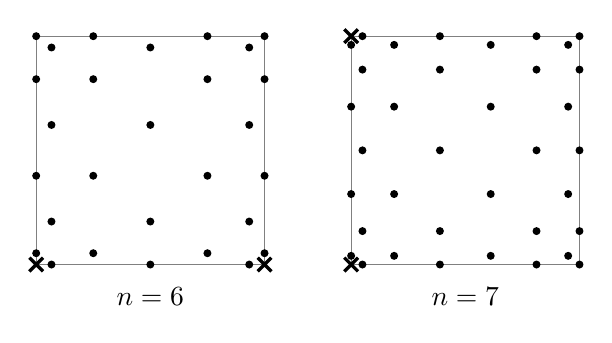
\begin{tikzpicture}[x=1.45cm,y=1.45cm]
\foreach \nn/\mm/\dx in {6/7/0,7/8/4} {
 \begin{scope}[xshift=\dx cm]
  \draw[gray] (-1,-1) rectangle (1,1);
  \foreach \jj in {0,...,\nn} {
   \foreach \kk in {0,...,\mm} {
    \pgfmathtruncatemacro{\parity}{mod(\jj+\kk,2)}
    \ifnum\parity=0
     \fill ({cos(180*\jj/\nn)},{cos(180*\kk/\mm)}) circle (0.035);
    \fi
   }
  }
  \draw[very thick] (-1.06,-1.06)--(-0.94,-0.94)
                    (-1.06,-0.94)--(-0.94,-1.06);
  \ifnum\nn=6
   \draw[very thick] (0.94,-1.06)--(1.06,-0.94)
                     (0.94,-0.94)--(1.06,-1.06);
  \else
   \draw[very thick] (-1.06,0.94)--(-0.94,1.06)
                     (-1.06,1.06)--(-0.94,0.94);
  \fi
  \node[below] at (0,-1.12) {$n=\nn$};
 \end{scope}
}
\end{tikzpicture}
\caption{The Padua points for two consecutive degrees. Dots are interpolation
points; crosses mark the two corners where the Lebesgue function attains
its maximum. The change of orientation depends only on parity.}
\label{fig:padua-nodes}
\end{figure}

Let $L_B$ be the cardinal polynomial associated with $B\in\mathcal P_n$.
Here \emph{cardinal polynomial} means the unique element of $\Pi_n$
whose value at $B$ is one and whose value at every other interpolation
node is zero. The collection of these polynomials is a basis adapted to
sampled values: a polynomial $p\in\Pi_n$ is reconstructed as
$p(z)=\sum_B p(B)L_B(z)$. In particular,
\[
 \sum_{B\in\mathcal P_n}L_B(z)=1,
\]
because the constant polynomial one is reproduced. Individual $L_B(z)$
can have either sign. The sum of their absolute values records how
large an arbitrary signed combination of the nodal data can become.
The Lebesgue function and its maximum are
\[
 \lambda_n(z)=\sum_{B\in\mathcal P_n}|L_B(z)|,
 \qquad \Lambda_n=\max_{z\in[-1,1]^2}\lambda_n(z).
\]
The function $\lambda_n$ is continuous, since it is a finite sum of
absolute values of polynomials. The square is compact, so the displayed
maximum exists. The identity $\sum_B L_B=1$ and the triangle inequality
give $\lambda_n(z)\geq1$ everywhere. At a node only one cardinal term
is nonzero, so there the lower bound is attained. This makes the values
between nodes especially relevant for stability.

For a real number $u$, the sign $\operatorname{sgn}u$ is $1$ when
$u>0$, $-1$ when $u<0$, and $0$ when $u=0$. At a fixed location
$z$, prescribe the data $e_B=\operatorname{sgn}L_B(z)$, choosing any
value of size at most one when a cardinal value is zero.
The corresponding interpolated value at $z$ is then exactly
$\sum_B|L_B(z)|$. Thus the absolute-value sum is the actual worst case
for bounded nodal data at that point. The sign choice can depend on $z$;
the Lebesgue function describes the worst case separately at each
location. Section~\ref{sec:preliminaries} also explains why these nodal
values may be extended to a continuous function of norm at most one,
which identifies $\Lambda_n$ with the operator norm on $C(Q)$.

At an interpolation point the Lebesgue function is exactly one. Away from
the points, its individual cardinal terms can reinforce each other.
For Padua interpolation the largest reinforcement occurs at the two corners
that are not interpolation points. This location was conjectured in
\cite{CaliariDeMarchiSommarivaVianello2008poster} and recorded among the
open problems in \cite[Section~3.3]{DeMarchi2022}.
Our first result identifies these maximizers exactly.

\begin{theorem}[Location of the maximum]\label{thm:main-location}
For every integer $n\geq2$, the maximum of $\lambda_n$ on the closed square
is attained exactly at
\[
 \begin{cases}
 \{(-1,-1),(1,-1)\},&n\text{ even},\\
 \{(-1,-1),(-1,1)\},&n\text{ odd}.
 \end{cases}
\]
In particular, $\Lambda_n=\Lambda_c(n)$, where
$\Lambda_c(n):=\lambda_n(-1,-1)$.
\end{theorem}

\noindent\textbf{The strength of the location assertion.}
An upper bound for $\Lambda_n$ would estimate the height of the graph
of $\lambda_n$. The theorem also determines all the locations reaching
that height. The word ``exactly'' includes the interior, all four edges,
the sampled points and every other corner: each point outside the
displayed pair has a strictly smaller value. This explains the need for
strict inequalities in the global argument. A dense plot can suggest
the two corners very convincingly, but the proof must control each
point of a continuum and must preserve equality information.

The equality between the values at the two listed corners comes from
a symmetry of the node set. For even $n$ the square can be reflected
in the vertical axis while preserving the nodes. For odd $n$ the
corresponding symmetry is reflection in the horizontal axis. Uniqueness
of interpolation transfers that geometric symmetry to $\lambda_n$.
The substantive global issue is the strict comparison with every other
point. Once it is resolved, a single scalar value
$\Lambda_c(n)=\lambda_n(-1,-1)$ determines the full norm.

The location proof is computer-assisted. Analytic estimates give the result
for $n\geq512$; rigorous finite certificates cover the remaining degrees.
The certificates bound the function on regions covering the square.
Sections~\ref{sec:argmax} and~\ref{sec:certificates} give these arguments
and their arithmetic assumptions.

Knowing the location reduces the Lebesgue constant to a single corner
value. Our second result describes that value much more precisely than
its leading growth rate. Here Euler's constant is
$\gamma=\lim_{R\to\infty}(H_R-\log R)$, where
$H_R=\sum_{r=1}^R r^{-1}$. Write
\begin{equation}\label{eq:main-constants}
 a=\frac2\pi,\qquad d=\gamma+\log\frac8\pi,\qquad
 c_1=ad,\qquad b=2ac_1,\qquad c=c_1^2+\kappa,
\end{equation}
with
\begin{equation}\label{eq:main-kappa}
 \kappa=\frac8\pi\int_0^1 t^2\cot\frac{\pi t}{2}
       \sum_{\substack{\ell\geq1\\\ell\text{ odd}}}
       \frac{1}{\ell(\ell^2-t^2)}\,dt.
\end{equation}
The apparent singularity at $t=1$ is canceled by the cotangent factor;
we justify convergence below.

\noindent\textbf{Reading the constants and the integral.}
The logarithms in this paper are natural logarithms. With $N=n+1/2$,
the letters in \eqref{eq:main-constants} package the coefficients of a square:
\[
 a^2\log^2N+b\log N+c
      =(a\log N+c_1)^2+\kappa
      =\frac4{\pi^2}(\log N+d)^2+\kappa.
\]
This identity is useful when tracing the two harmonic sums in the
corner calculation. Each has a logarithmic leading term and a constant
term. Multiplying them produces the squared logarithm, a single
logarithm and a constant. The coupled part of the calculation supplies
the additional constant $\kappa$.

The sum in \eqref{eq:main-kappa} runs over the positive odd integers
$1,3,5,\ldots$. The $\ell=1$ term deserves separate attention near
$t=1$. For every $0\leq t\leq1$ and integer $\ell\geq3$,
\[
 \ell^2-t^2\geq\ell^2-1\geq\frac89\ell^2,
 \qquad
 0\leq\frac1{\ell(\ell^2-t^2)}\leq\frac9{8\ell^3}.
\]
The last bound has a convergent sum: for example,
$\sum_{\ell=L}^{\infty}\ell^{-3}$ is at most
$L^{-3}+\int_L^{\infty}x^{-3}\,dx=L^{-3}+1/(2L^2)$.
It follows that the tail of the series over odd $\ell\geq3$ is
bounded by a quantity tending to zero independently of $t$. This is
uniform convergence on $[0,1]$. Each summand is continuous there, so
this part of the sum is a bounded continuous function, including both
endpoints. The remaining term, $\ell=1$, is handled separately.
Near $t=0$,
$\cot(\pi t/2)$ is of size $1/t$, so the factor $t^2$ makes the
complete integrand of size $t$. Near $t=1$ the potentially singular
term contains
\[
 \frac{t^2\cot(\pi t/2)}{1-t^2},
 \qquad
 \lim_{t\uparrow1}
 \frac{t^2\cot(\pi t/2)}{1-t^2}=\frac\pi4.
\]
Indeed, $\cot(\pi t/2)=\tan(\pi(1-t)/2)$ and
$1-t^2=(1-t)(1+t)$. These elementary endpoint checks already explain
why the integral specifies a finite real number. The later proof gives
the precise estimates needed for its use in the asymptotic expansion.

\begin{theorem}[Sharp corner expansion]\label{thm:main-expansion}
Let $N=n+\tfrac12$. For the points \eqref{eq:nodes}, as $n\to\infty$,
\begin{equation}\label{eq:main-expansion}
 \Lambda_c(n)=\frac4{\pi^2}\log^2N+b\log N+c-\frac1N
            +O\!\left(\frac{\log N}{N^2}\right).
\end{equation}
The constants and the remainder estimate are the same for both parities.
More precisely, a finite constant $C$, independent of $n$, bounds the
absolute remainder by $C\log N/N^2$ for every integer $n\geq2$.
Consequently \eqref{eq:main-expansion} also holds for $\Lambda_n$.
\end{theorem}

\noindent\textbf{What the error term says.}
If $\mathcal{R}_n$ denotes the difference between $\Lambda_c(n)$ and the four
explicit terms in \eqref{eq:main-expansion}, the statement is
\[
 |\mathcal{R}_n|\leq C\frac{\log(n+1/2)}{(n+1/2)^2}
 \quad(n\geq2)
\]
for one finite constant $C$ that works for every degree and both
parities. In particular $N \mathcal{R}_n\to0$. The remainder is smaller than $1/N$, so the coefficient of
the reciprocal term $-1/N$ is determined. A leading
$O(\log n)$ estimate leaves the constant and reciprocal terms
undetermined. The content of the sharp expansion lies in keeping
track of contributions small enough to affect those terms.

The change from $n$ to $N=n+1/2$ also matters at this accuracy. For
example, elementary Taylor expansion gives
\[
 \log(n+\tfrac12)=\log n+\frac1{2n}+O(n^{-2}),
 \qquad
 \log^2(n+\tfrac12)=\log^2n+\frac{\log n}{n}
                         +O\!\left(\frac{\log n}{n^2}\right).
\]
The correction $(\log n)/n$ is larger than the final remainder in the
theorem. A shift of scale therefore changes the lower-order bookkeeping.
The scale $N$ absorbs the logarithmic reciprocal term, leaving the pure
$-1/N$ correction. Both parities share one formula at each of the scales
$n$, $m=n+1$ and $N=n+1/2$.

An asymptotic expansion describes the behavior along arbitrarily large
degrees. The theorem additionally states a uniform bound for every
$n\geq2$. As usual, once the tail estimate is proved, finitely many
remaining degrees can be absorbed by increasing a finite constant.
That observation concerns the remainder bound for the corner value;
the separate global location theorem still has its own pointwise proof.

The corner expansion is proved analytically. Its transfer to $\Lambda_n$
as $n\to\infty$ uses only the analytic $n\geq512$ part of
Theorem~\ref{thm:main-location}. The finite certificates also identify the
maximum in the remaining degrees; the same remainder constant can therefore
be chosen for all $n\geq2$.

The leading growth
$\Lambda_n=(4/\pi^2)\log^2n+O(\log n)$ is due to
Kolomoitsev and Lomako~\cite[Theorem~2.1 and the following Padua consequence]{KolomoitsevLomako2021}.
Their proof uses pointwise rhombic Lebesgue-function asymptotics of
Kuznetsova~\cite[Theorem~1]{Kuznetsova1995}; Pimenova's earlier equal-parameter
result concerns the corresponding odd periodic grid
\cite[Theorem~1]{Pimenova1979}. These periodic results form the background
for the leading Padua asymptotics.

The lower-order sizes had also been anticipated numerically. De Marchi's
empirical model was $((2/\pi)\log(n+1)+1.1)^2$
\cite[Section~1.1, pp.~3--5]{DeMarchi2005NearOptimal}.
Here the explicit constants are
$b\approx1.225522125742$, $c\approx1.846160310424$, and
$\kappa\approx0.919710118388$. Theorem~\ref{thm:main-expansion}
identifies their exact expressions and resolves the lower terms through
an error smaller than $1/n$. Its square
comes from two harmonic sums; $\kappa$ measures their coupling, and the
half-integer scale exposes the reciprocal correction.

Both proofs begin with the same corrected interpolation kernel. At the
corner its signs give an exact positive sum. Away from the corner, reflection
writes the Lebesgue function as a periodic envelope minus the cancellation
lost in taking absolute values. A single comparison with a completed model
then controls that envelope and the competing reflection defects. Near an
actual maximizing corner, a positive interpolation argument proves strict
quadratic descent. The finite certificates use that same interpolation
principle. This organization separates the two ideas that matter: computing
the corner value and showing why no other point can exceed it.

Here the \emph{envelope} is an explicit upper-bound function obtained
by taking absolute values of reflected kernel terms before combining
them. It is periodic in angular coordinates. A \emph{reflection defect}
is the amount by which that upper bound exceeds the value after the
signed terms have been combined; it measures the cancellation lost in
the triangle inequality. The \emph{completed model} is an auxiliary
comparison expression, defined in the global argument, that allows us
to estimate the finite envelope by isolating its common large-degree
behavior and controlling the remaining error.

A \emph{positive interpolation argument} uses nonnegative interpolation
weights to carry bounds on finitely many values over an entire region,
with a proved remainder bound when the interpolation is approximate.
For example, a convex combination of four vertex values cannot exceed
their largest value. This positivity belongs to the interpolation
weights in the comparison argument; the Padua cardinal polynomials
introduced above can have either sign. Finally, \emph{quadratic descent}
means that sufficiently near a maximizing corner the loss from the
corner value is bounded below by a positive constant times squared
angular displacement. Such a bound is strictly positive at every
nearby point with nonzero displacement and vanishes at the corner.

The Padua construction and its generating-curve and ideal descriptions
are classical~\cite{BosCaliariDeMarchiVianelloXu2006,BosDeMarchiVianelloXu2007}.
Related numerical geometry of local maxima is studied in
\cite{BialasCiezDeMarchiSuder2026}. Rigorous norm approximation by polynomial
meshes, including Padua examples, was developed in~\cite{Mesh2024}; our
certificates add strict exclusion near the maximizing corners, identifying
the equality set.
For the distinct Morrow--Patterson family,
\cite{MorrowPatterson2026} proves an $O(n^2)$ upper bound.

We derive the corner expansion in Section~\ref{sec:corner}, then establish
one comparison theorem and apply it to the global location in
Section~\ref{sec:argmax}. Section~\ref{sec:certificates} completes the finite
range and states the arithmetic and evidence dependencies.


\noindent\textbf{A route through the proof.}
The normalization section begins with finite-dimensional linear algebra.
It proves that the node values uniquely determine a polynomial and
derives the cardinal polynomials from a weighted scalar product. This
step fixes the coefficient of one exceptional highest-frequency term;
all subsequent numerical constants refer to that normalization.
The angular variables then turn the polynomial kernel into finite cosine
sums. Geometric-series identities and elementary trigonometry are the
basic tools for making those sums explicit.

The corner section evaluates those sums where their signs can be
organized exactly. It isolates the harmonic growth, the coupled integral
and the endpoint corrections. Keeping endpoint terms matters because
their total contribution can be of order $1/n$, the scale resolved by
the second theorem. The global comparison section instead studies
points throughout the square. There absolute values hide some of the
signed cancellation, so the proof measures that cancellation explicitly
and compares it with the available envelope bound. The finite-row
estimates quantify the comparison uniformly across the required regions.

Finally, the certificate section explains how polynomial bounds on
closed regions yield global strict inequalities. Closed regions may
overlap along their boundaries; including those boundaries makes the
cover complete. Regions containing a maximizing corner require an
equality-aware argument, since the upper bound is attained there.
The proof has two obligations: evaluate the corner value and exclude
every competing point. The corner expansion and the global comparison
address these two obligations.

The explanations below develop each construction when it is first
needed. The numbered statements and formulas retain the same roles
throughout: they specify the quantitative results to be proved, while
the intervening derivations explain the linear algebra, trigonometric
identities and estimates on which those results depend.
